\documentclass[12pt,a4paper]{article}

\input{preamble}

\begin{document}

% ============================================================
% PAGE DE GARDE
% ============================================================

\begin{titlepage}
    \centering

    \vspace*{1.5cm}

    {\Large Université Nice Côte d'Azur\par}

    \vspace{0.3cm}

    {\large EUR DS4H -- Master 2 ESTel\par}

    \vspace{2.5cm}

    {\Huge\bfseries TP 1\par}

    \vspace{0.5cm}

    {\LARGE\bfseries Étude de la consommation d'un core\par}

    \vspace{1.5cm}

    {\Large Architecture multicores\par}

    \vfill

    \begin{tabular}{rl}
        \textbf{FPGA :} & Cyclone V \\
        \textbf{Référence :} & 5CSEBA6U23I7 \\
        \textbf{Logiciel :} & Quartus Prime Lite 17.1 \\
    \end{tabular}

    \vfill

    {\large Année universitaire 2026--2027\par}

\end{titlepage}


% ============================================================
% SOMMAIRE
% ============================================================

\tableofcontents

\newpage


% ============================================================
% INTRODUCTION
% ============================================================

\section{Introduction}

L'objectif de ce TP est d'étudier la consommation énergétique
d'opérateurs arithmétiques implantés sur FPGA et d'observer
l'influence de différents paramètres architecturaux, notamment
la fréquence de fonctionnement et la profondeur du pipeline.

Les différentes architectures sont synthétisées avec Quartus Prime
Lite 17.1 pour un FPGA Cyclone V 5CSEBA6U23I7.

La consommation est estimée à l'aide de l'outil
\textit{Power Analyzer} de Quartus. Les analyses présentées dans
ce rapport utilisent l'estimation d'activité \textit{Vectorless}.


% ============================================================
% EXERCICE 1
% ============================================================

\section{Opérateurs et consommation}


% ============================================================
% ADDITION ENTIERE
% ============================================================

\subsection{Addition entière 32 bits}

Dans un premier temps, un additionneur entier 32 bits a été étudié.
L'opérateur a été réalisé à l'aide du bloc
\texttt{LPM\_ADD\_SUB} de Quartus.

Les deux entrées $A$ et $B$ sont codées sur 32 bits et
l'opération réalisée est une addition signée.

Afin d'étudier l'influence du pipeline, trois profondeurs ont été
considérées :

\begin{itemize}
    \item pipeline 1 ;
    \item pipeline 2 ;
    \item pipeline 4.
\end{itemize}


% ============================================================
% FIGURES ADDITION ENTIERE
% ============================================================

\subsubsection{Architectures étudiées}

La Figure~\ref{fig:addition_pipeline} présente les trois
configurations réalisées sous Quartus.

\begin{figure}[H]
    \centering

    \begin{subfigure}[b]{0.32\textwidth}
        \centering
        \includegraphics[width=\textwidth]
        {addition_entier_pipeline1.png}
        \caption{Pipeline 1}
        \label{fig:add_p1}
    \end{subfigure}
    \hfill
    \begin{subfigure}[b]{0.32\textwidth}
        \centering
        \includegraphics[width=\textwidth]
        {addition_entier_pipeline2.png}
        \caption{Pipeline 2}
        \label{fig:add_p2}
    \end{subfigure}
    \hfill
    \begin{subfigure}[b]{0.32\textwidth}
        \centering
        \includegraphics[width=\textwidth]
        {addition_entier_pipeline4.png}
        \caption{Pipeline 4}
        \label{fig:add_p4}
    \end{subfigure}

    \caption{Additionneur entier 32 bits pour les différentes
    profondeurs de pipeline étudiées.}

    \label{fig:addition_pipeline}
\end{figure}


% ============================================================
% FREQUENCES
% ============================================================

\subsubsection{Fréquences de fonctionnement}

La fréquence d'horloge a été adaptée en fonction de la fréquence
maximale obtenue avec l'outil TimeQuest.

Pour le pipeline 1, TimeQuest n'a retourné aucun chemin permettant
d'obtenir une fréquence maximale exploitable. Une fréquence de
100 MHz a donc été conservée comme fréquence d'étude.

\begin{table}[H]
    \centering
    \caption{Fréquences utilisées pour l'addition entière}

    \begin{tabular}{ccc}
        \toprule
        \textbf{Pipeline} &
        \textbf{Fréquence} &
        \textbf{Origine} \\
        \midrule

        1 & 100 MHz & Fréquence d'étude \\
        2 & 337,27 MHz & TimeQuest \\
        4 & 210,70 MHz & TimeQuest \\

        \bottomrule
    \end{tabular}
\end{table}


% ============================================================
% CONSOMMATION ENTIERE
% ============================================================

\subsubsection{Consommation}

Les résultats obtenus avec Power Analyzer sont présentés dans le
Tableau~\ref{tab:power_integer}.

\begin{table}[H]
    \centering

    \caption{Consommation de l'additionneur entier 32 bits}

    \label{tab:power_integer}

    \begin{tabular}{ccccc}
        \toprule

        \textbf{Pipeline} &
        \textbf{Fréquence} &
        \textbf{$P_{tot}$} &
        \textbf{$P_{dyn}$} &
        \textbf{$P_{stat}$} \\

        \midrule

        1 & 100 MHz
          & 441,43 mW
          & 1,15 mW
          & 412,36 mW \\

        2 & 337,27 MHz
          & 490,76 mW
          & 5,52 mW
          & 412,77 mW \\

        4 & 210,70 MHz
          & 476,23 mW
          & 3,91 mW
          & 412,65 mW \\

        \bottomrule
    \end{tabular}
\end{table}


% ============================================================
% ENERGIE PAR OPERATION
% ============================================================

\subsubsection{Énergie par opération}

Une fois le pipeline rempli, l'architecture peut fournir une
opération par cycle d'horloge.

L'énergie moyenne consommée par opération est donc estimée par :

\begin{equation}
    E_{op} = \frac{P}{f}
\end{equation}

où $P$ représente la puissance consommée et $f$ la fréquence
de fonctionnement.

Une fenêtre d'observation de 1000 opérations en régime établi
est considérée. Sur cette durée, le coût associé au remplissage
initial du pipeline devient négligeable.

\begin{table}[H]
    \centering

    \caption{Énergie par opération pour l'addition entière}

    \begin{tabular}{ccc}
        \toprule

        \textbf{Pipeline} &
        \textbf{$E_{tot}/op$} &
        \textbf{$E_{dyn}/op$} \\

        \midrule

        1 & 4,414 nJ/op & 11,50 pJ/op \\
        2 & 1,455 nJ/op & 16,37 pJ/op \\
        4 & 2,260 nJ/op & 18,56 pJ/op \\

        \bottomrule
    \end{tabular}
\end{table}

Parmi les configurations étudiées, le pipeline 2 présente
l'énergie totale par opération la plus faible.


% ============================================================
% ADDITION FLOTTANTE
% ============================================================

\subsection{Addition flottante 32 bits}

L'étude est ensuite réalisée avec un additionneur flottant 32 bits
à l'aide du bloc \texttt{ALTFP\_ADD\_SUB}.

Les paramètres utilisés sont :

\begin{itemize}
    \item largeur de l'exposant : 8 bits ;
    \item largeur de la mantisse : 23 bits ;
    \item pipeline : 14 étages ;
    \item arrondi : \textit{To Nearest}.
\end{itemize}

Le pipeline proposé par l'IP est conservé.


% ============================================================
% FIGURE FLOAT
% ============================================================

La Figure~\ref{fig:add_float} présente l'architecture réalisée
dans Quartus.

\begin{figure}[H]
    \centering

    \includegraphics[
        width=0.88\textwidth
    ]{addition_flottant_pipeline14.png}

    \caption{Additionneur flottant 32 bits avec un pipeline
    de 14 étages.}

    \label{fig:add_float}
\end{figure}


% ============================================================
% RESULTATS FLOAT
% ============================================================

L'analyse temporelle avec TimeQuest donne une fréquence maximale
conservatrice de :

\begin{equation}
    f_{\max} = 183,82~\text{MHz}
\end{equation}

À cette fréquence, les résultats obtenus sont :

\begin{table}[H]
    \centering

    \caption{Résultats de l'additionneur flottant 32 bits}

    \begin{tabular}{lc}
        \toprule

        \textbf{Paramètre} &
        \textbf{Valeur} \\

        \midrule

        Pipeline & 14 \\
        Fréquence & 183,82 MHz \\
        Puissance totale & 467,32 mW \\
        Puissance dynamique du coeur & 16,48 mW \\
        Puissance statique & 412,61 mW \\
        Énergie totale par opération & 2,542 nJ/op \\
        Énergie dynamique par opération & 89,65 pJ/op \\

        \bottomrule
    \end{tabular}
\end{table}


% ============================================================
% FREQUENCE / PUISSANCE
% ============================================================

\subsection{Influence de la fréquence sur la puissance}

Afin d'étudier directement l'influence de la fréquence,
le même additionneur flottant pipeline 14 a également été
analysé à une fréquence de 100 MHz.

\begin{table}[H]
    \centering

    \caption{Influence de la fréquence sur la consommation
    de l'additionneur flottant}

    \begin{tabular}{ccc}
        \toprule

        \textbf{Fréquence} &
        \textbf{$P_{dyn}$} &
        \textbf{$P_{tot}$} \\

        \midrule

        100 MHz
        & 8,97 mW
        & 448,09 mW \\

        183,82 MHz
        & 16,48 mW
        & 467,32 mW \\

        \bottomrule
    \end{tabular}
\end{table}

La puissance dynamique d'un circuit numérique peut être
approximée par :

\begin{equation}
    P_{dyn} \approx \alpha C V^2 f
\end{equation}

où :

\begin{itemize}
    \item $\alpha$ représente l'activité de commutation ;
    \item $C$ représente la capacité équivalente commutée ;
    \item $V$ représente la tension d'alimentation ;
    \item $f$ représente la fréquence de fonctionnement.
\end{itemize}

Lorsque la fréquence passe de 100 MHz à 183,82 MHz,
la puissance dynamique passe de 8,97 mW à 16,48 mW.

La fréquence augmente d'environ 84\,\% et la puissance dynamique
augmente dans des proportions comparables.

L'augmentation de la fréquence permet donc d'augmenter le débit
de calcul, mais entraîne également une augmentation de la
puissance dynamique.


% ============================================================
% INFLUENCE PIPELINE
% ============================================================

\subsection{Influence du pipeline}

Le pipeline consiste à découper le chemin combinatoire d'un
opérateur en plusieurs étages séparés par des registres.

En théorie, cette technique permet de réduire la longueur du
chemin critique entre deux registres et peut donc permettre
d'augmenter la fréquence maximale de fonctionnement.

Les résultats obtenus pour l'addition entière donnent cependant :

\begin{table}[H]
    \centering

    \caption{Influence du pipeline sur la fréquence maximale}

    \begin{tabular}{cc}
        \toprule

        \textbf{Pipeline} &
        \textbf{Fréquence} \\

        \midrule

        2 & 337,27 MHz \\
        4 & 210,70 MHz \\

        \bottomrule
    \end{tabular}
\end{table}


Dans notre implémentation, le pipeline 4 n'atteint donc pas une
fréquence supérieure au pipeline 2.

L'augmentation de la profondeur du pipeline ne garantit donc pas
une augmentation systématique de la fréquence maximale après
synthèse et placement-routage.

Les performances finales dépendent également de l'architecture
générée par l'IP, du placement-routage et des chemins critiques
obtenus.

\begin{figure}[H]
\centering
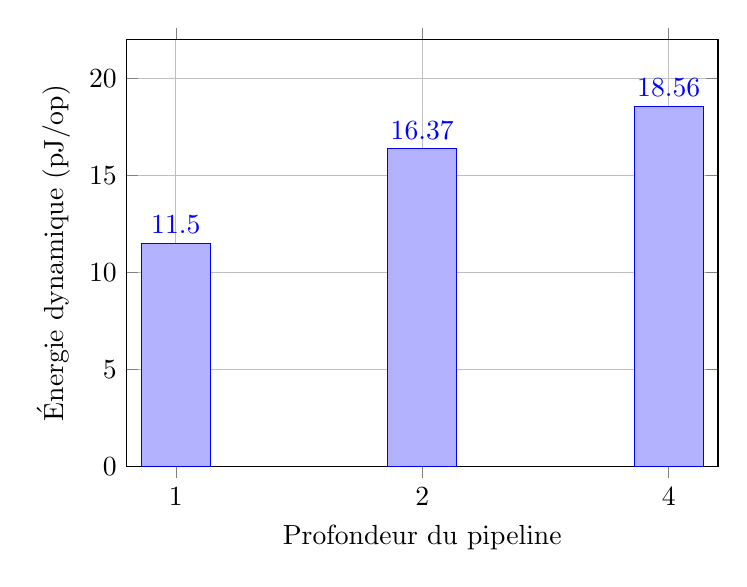
\begin{tikzpicture}
\begin{axis}[
    ybar,
    width=0.75\textwidth,
    height=7cm,
    ylabel={Énergie dynamique (pJ/op)},
    xlabel={Profondeur du pipeline},
    symbolic x coords={1,2,4},
    xtick=data,
    ymin=0,
    ymax=22,
    nodes near coords,
    nodes near coords align={vertical},
    grid=major,
    bar width=25pt
]

\addplot coordinates {
    (1,11.50)
    (2,16.37)
    (4,18.56)
};

\end{axis}
\end{tikzpicture}
\caption{Énergie dynamique par opération de l'additionneur entier
32 bits en fonction de la profondeur du pipeline.}
\label{fig:energie_dyn_entier}
\end{figure}


% ============================================================
% ENTIER VS FLOAT
% ============================================================

\subsection{Comparaison entre calcul entier et flottant}

Une addition flottante est plus complexe qu'une addition entière.

Elle nécessite notamment :

\begin{itemize}
    \item le traitement des exposants ;
    \item l'alignement des mantisses ;
    \item l'addition ;
    \item la normalisation ;
    \item l'arrondi du résultat.
\end{itemize}

Cette complexité supplémentaire apparaît dans l'énergie dynamique
consommée par opération.

\begin{table}[H]
    \centering

    \caption{Comparaison de l'énergie dynamique par opération}

    \begin{tabular}{ccc}
        \toprule

        \textbf{Type} &
        \textbf{Pipeline} &
        \textbf{$E_{dyn}/op$} \\

        \midrule

        Entier & 1 & 11,50 pJ/op \\
        Entier & 2 & 16,37 pJ/op \\
        Entier & 4 & 18,56 pJ/op \\
        Flottant & 14 & 89,65 pJ/op \\

        \bottomrule
    \end{tabular}
\end{table}

L'addition flottante présente donc un coût énergétique dynamique
nettement supérieur à celui des additions entières étudiées.

\begin{figure}[H]
\centering
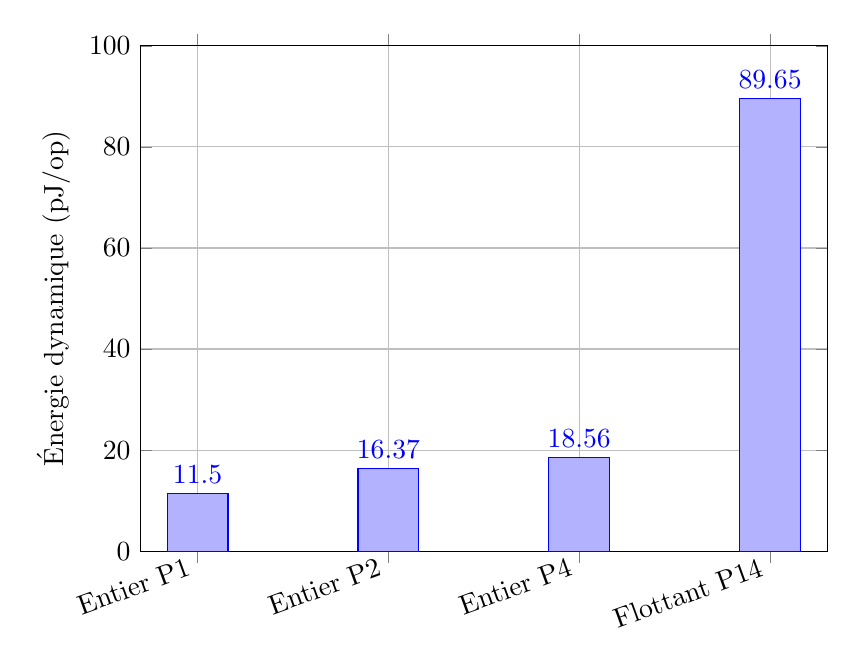
\begin{tikzpicture}
\begin{axis}[
    ybar,
    width=0.85\textwidth,
    height=8cm,
    ylabel={Énergie dynamique (pJ/op)},
    symbolic x coords={Entier P1,Entier P2,Entier P4,Flottant P14},
    xtick=data,
    x tick label style={rotate=20,anchor=east},
    ymin=0,
    ymax=100,
    nodes near coords,
    nodes near coords align={vertical},
    grid=major,
    bar width=22pt
]

\addplot coordinates {
    (Entier P1,11.50)
    (Entier P2,16.37)
    (Entier P4,18.56)
    (Flottant P14,89.65)
};

\end{axis}
\end{tikzpicture}
\caption{Comparaison de l'énergie dynamique par opération
des additionneurs entier et flottant.}
\label{fig:energie_dyn_comparaison}
\end{figure}


% ============================================================
% MULTIPLICATEUR
% ============================================================

\subsection{Étude du multiplicateur 32 bits}

Un multiplicateur signé 32 bits a ensuite été étudié à l'aide du
bloc \texttt{LPM\_MULT} de Quartus. Les deux entrées $A$ et $B$
sont codées sur 32 bits et le résultat de la multiplication est
fourni sur 64 bits.

La Figure~\ref{fig:mult32} présente l'architecture réalisée sous
Quartus pour le multiplicateur avec un pipeline de profondeur 1.

\begin{figure}[H]
    \centering
    \includegraphics[width=0.88\textwidth]
    {multiplicateur_pipeline1.png}
    \caption{Multiplicateur signé 32 bits réalisé avec
    \texttt{LPM\_MULT}, pipeline 1.}
    \label{fig:mult32}
\end{figure}

Trois profondeurs de pipeline ont été étudiées :

\begin{itemize}
    \item pipeline 1 ;
    \item pipeline 2 ;
    \item pipeline 4.
\end{itemize}

Après synthèse, Quartus utilise trois blocs DSP pour réaliser
la multiplication 32 bits dans les configurations étudiées.

\subsubsection{Ressources utilisées}

\begin{table}[H]
    \centering
    \caption{Ressources utilisées par le multiplicateur}

    \begin{tabular}{cccc}
        \toprule
        \textbf{Pipeline} &
        \textbf{ALMs} &
        \textbf{Registres} &
        \textbf{DSP} \\
        \midrule
        1 & 24 & 0   & 3 \\
        2 & 24 & 0   & 3 \\
        4 & 46 & 161 & 3 \\
        \bottomrule
    \end{tabular}
\end{table}

Le nombre de blocs DSP reste constant pour les trois configurations.
En revanche, le pipeline 4 entraîne une augmentation des ressources
logiques et utilise 161 registres.

\subsubsection{Consommation du multiplicateur}

\begin{table}[H]
    \centering
    \caption{Consommation du multiplicateur utilisant les blocs DSP}

    \begin{tabular}{ccccc}
        \toprule
        \textbf{Pipeline} &
        \textbf{$P_{tot}$} &
        \textbf{$P_{dyn}$} &
        \textbf{$P_{stat}$} &
        \textbf{I/O} \\
        \midrule
        1 & 532,58 mW & 8,23 mW & 413,13 mW & 111,22 mW \\
        2 & 530,84 mW & 6,50 mW & 413,11 mW & 111,22 mW \\
        4 & 532,81 mW & 8,72 mW & 413,13 mW & 110,96 mW \\
        \bottomrule
    \end{tabular}
\end{table}

La puissance totale varie peu entre les trois configurations et
reste comprise entre 530,84 mW et 532,81 mW.

La puissance dynamique du coeur varie davantage. Elle est de
8,23 mW pour le pipeline 1, 6,50 mW pour le pipeline 2 et
8,72 mW pour le pipeline 4.

Dans les conditions de cette estimation, le pipeline 2 présente
donc la puissance dynamique la plus faible parmi les trois
configurations étudiées.


% ============================================================
% RESSOURCES MULTIPLICATEUR
% ============================================================

\subsubsection{Ressources utilisées}

\begin{table}[H]
    \centering

    \caption{Ressources utilisées par le multiplicateur DSP}

    \begin{tabular}{cccc}
        \toprule

        \textbf{Pipeline} &
        \textbf{ALMs} &
        \textbf{Registres} &
        \textbf{DSP} \\

        \midrule

        1 & 24 & 0 & 3 \\
        2 & 24 & 0 & 3 \\
        4 & 46 & 161 & 3 \\

        \bottomrule
    \end{tabular}
\end{table}

Les trois configurations utilisent trois blocs DSP.

Le pipeline 4 nécessite cependant davantage de ressources logiques
avec 46 ALMs et 161 registres.


% ============================================================
% POWER MULTIPLICATEUR
% ============================================================

\subsubsection{Consommation du multiplicateur}

\begin{table}[H]
    \centering

    \caption{Consommation du multiplicateur utilisant les blocs DSP}

    \begin{tabular}{ccccc}
        \toprule

        \textbf{Pipeline} &
        \textbf{$P_{tot}$} &
        \textbf{$P_{dyn}$} &
        \textbf{$P_{stat}$} &
        \textbf{I/O} \\

        \midrule

        1 &
        532,58 mW &
        8,23 mW &
        413,13 mW &
        111,22 mW \\

        2 &
        530,84 mW &
        6,50 mW &
        413,11 mW &
        111,22 mW \\

        4 &
        532,81 mW &
        8,72 mW &
        413,13 mW &
        110,96 mW \\

        \bottomrule
    \end{tabular}
\end{table}

La puissance totale varie relativement peu entre les trois
configurations et reste comprise entre environ 530,8 mW et
532,8 mW.

La puissance dynamique est davantage affectée par le pipeline.
Elle vaut 8,23 mW pour le pipeline 1, 6,50 mW pour le pipeline 2
et 8,72 mW pour le pipeline 4.

Dans les conditions de cette estimation, le pipeline 2 présente
donc la puissance dynamique la plus faible parmi les trois
configurations étudiées.


% ============================================================
% DISCUSSION
% ============================================================

\subsection{Discussion des résultats}

Les différentes mesures mettent en évidence l'existence d'un
compromis entre fréquence de fonctionnement, profondeur du pipeline,
ressources matérielles et consommation.

L'augmentation de la fréquence permet d'augmenter le nombre
d'opérations pouvant être réalisées par seconde. En contrepartie,
elle augmente l'activité de commutation du circuit et donc sa
puissance dynamique.

Ce comportement apparaît clairement avec l'additionneur flottant :
la puissance dynamique passe de 8,97 mW à 100 MHz à 16,48 mW
à 183,82 MHz.

Le pipeline permet théoriquement de réduire les chemins
combinatoires entre les registres et donc de faciliter
l'augmentation de la fréquence maximale.

Cependant, les résultats obtenus montrent que cette évolution
n'est pas nécessairement monotone après synthèse et
placement-routage. L'additionneur entier pipeline 2 atteint
337,27 MHz alors que le pipeline 4 atteint 210,70 MHz.

Il ne faut donc pas conclure qu'une augmentation systématique
du nombre d'étages de pipeline conduit nécessairement à une
fréquence maximale supérieure.

Enfin, l'addition flottante présente un coût énergétique dynamique
plus important que l'addition entière en raison de la complexité
supérieure des opérations nécessaires à son implémentation.


% ============================================================
% LIMITES
% ============================================================

\subsection{Limites des estimations}

Toutes les mesures de puissance présentées ont été obtenues avec
l'estimation d'activité \textit{Vectorless} de Power Analyzer.

Quartus indique :

\begin{center}
    \texttt{Power Estimation Confidence : Low}
\end{center}

Cette indication est liée à l'absence de données précises sur
l'activité réelle de commutation des différents signaux.

Les valeurs absolues de puissance doivent donc être considérées
comme des estimations.

Cependant, l'utilisation de la même méthode et des mêmes conditions
d'analyse pour les différentes architectures permet d'effectuer
une comparaison cohérente de leurs tendances de consommation.


% ============================================================
% CONCLUSION EXERCICE 1
% ============================================================

\subsection{Conclusion de l'exercice}

Cette étude montre que l'augmentation de la fréquence permet
d'améliorer le débit de calcul mais entraîne également une
augmentation de la puissance dynamique.

Le pipeline peut permettre d'augmenter la fréquence maximale en
réduisant la longueur des chemins combinatoires. Cependant, les
résultats obtenus montrent que l'ajout d'étages supplémentaires
ne garantit pas systématiquement une fréquence maximale plus élevée
après synthèse et placement-routage.

Dans notre étude, l'additionneur entier pipeline 2 atteint
337,27 MHz et présente une énergie totale de 1,455 nJ par opération,
alors que le pipeline 4 atteint 210,70 MHz pour 2,260 nJ par
opération.

L'addition flottante présente quant à elle une consommation
dynamique et une énergie dynamique par opération nettement
supérieures à celles des additions entières.

Le choix d'une architecture doit donc prendre en compte plusieurs
critères simultanément : la fréquence maximale, le débit de calcul,
la consommation dynamique, l'énergie par opération et les ressources
matérielles utilisées.


% ============================================================
% EXERCICE 2
% ============================================================

\newpage

\section{Application à un cas d'étude : filtre vidéo}

% À compléter lors de l'exercice 2.


% ============================================================
% EXERCICE 3
% ============================================================

\newpage

\section{Mesure sur plateforme FPGA}

% À compléter lors de l'exercice 3.


% ============================================================
% CONCLUSION GENERALE
% ============================================================

\newpage

\section{Conclusion générale}

% À compléter après les exercices 2 et 3.


\end{document}